\subsection{Computation of natural frequencies}
\label{subsec:natural_frequencies}

From theory, we know that the natural frequencies of a system can be computed by solving the following eigenvalue problem:

\begin{equation}
    det(H(\omega_n)) = 0
\end{equation}

Where $H(\omega_n)$ is the transfer function of the system as reported in Equation \ref{eq:linear_system} and $\omega_n$ is one of the natural frequencies.

By iterating over a given vector of frequencies, we can compute the value of the determinant of the matrix $H(\omega)$ and find the minimums, which correspond to the natural frequencies of the system.

The result of this computation is shown in Figure \ref{fig:natural_frequencies}.

\begin{figure}[H]
    \centering
    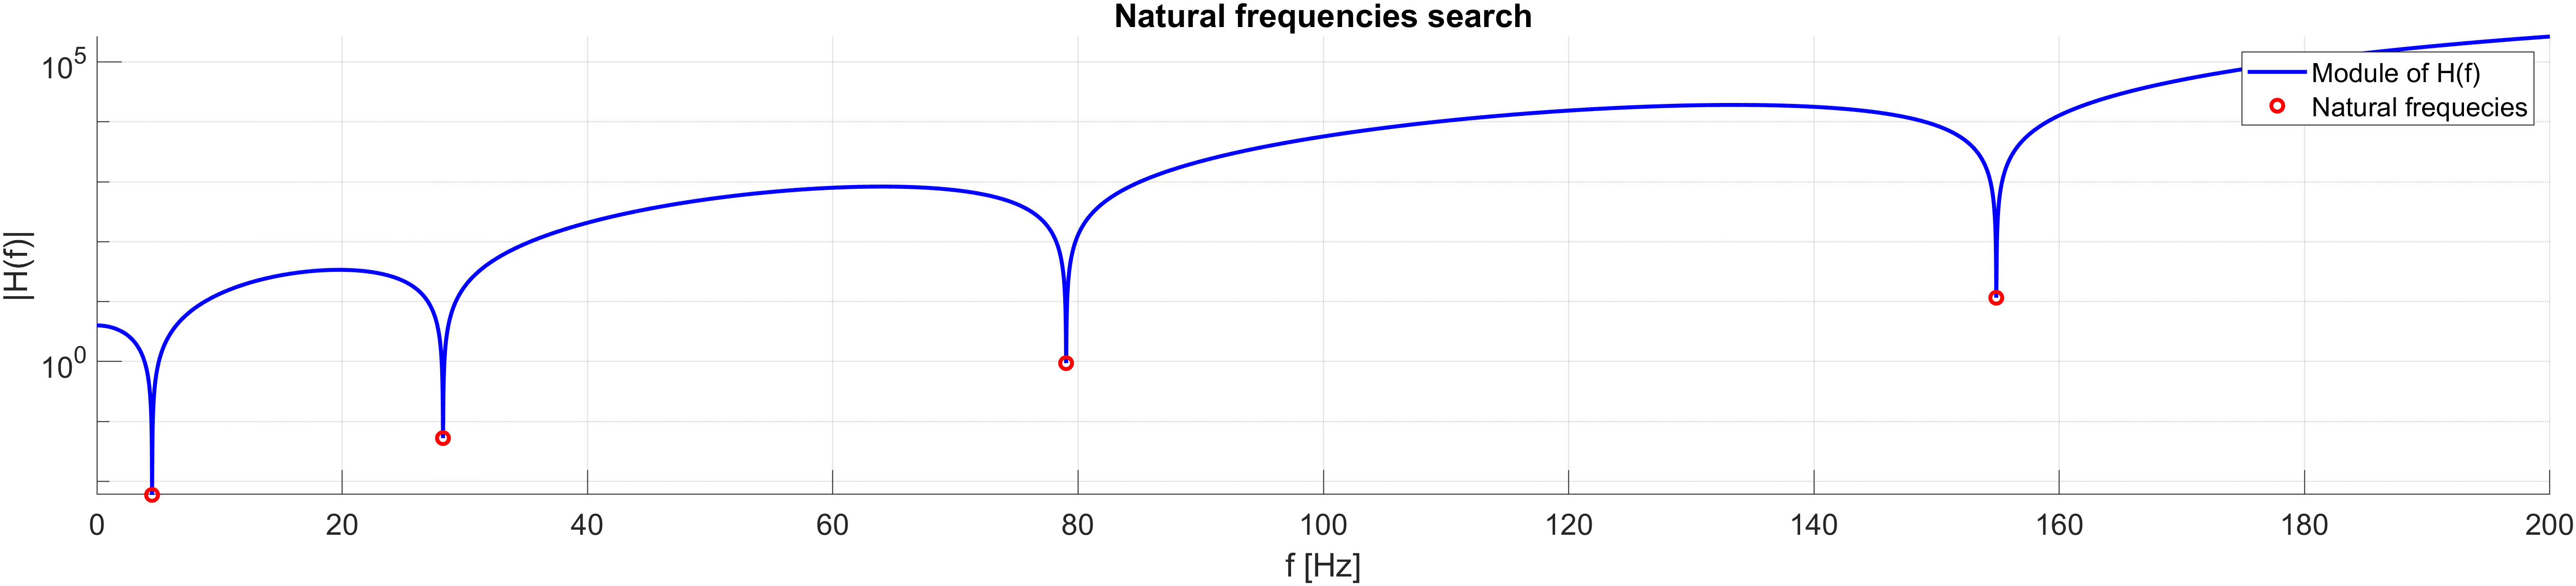
\includegraphics[width=\textwidth]{img/MATLAB/Part_A/H_module.png}
    \caption{Numerical search for natural frequencies of the system. Minimums value of $det[H(\omega)]$ are considered as natural frequencies.}
    \label{fig:natural_frequencies}
\end{figure}
